\documentclass[letterpaper]{article}
\usepackage{times}
\usepackage{helvet}
\usepackage{courier}
\usepackage{graphicx}
\usepackage{enumerate}
\usepackage{amssymb}
\usepackage{amsmath}
\DeclareMathOperator*{\argmax}{argmax}

\title{HUBzero Test Environment}
%\author{Derrick S. Kearney \\
%\texttt{dsk@purdue.edu} \\
%\\
%Purdue University \\
%West Lafayette, IN 47909}

\begin{document}
\maketitle

\begin{abstract}
The HUBzero software stack is comprised of several pieces (web, middleware,
tools) that are usually developed individually even though they are built to
work together. The autonomous nature of the software development cycle
encourages software testing that is self-reliant. Changes to designs,
protocols, and settings happen without the knowledge of developers from
other pieces of the hub. This practice invalidates knowledge of how the hub
works, contradicts documentation, and provides the opportunity to break
seemingly unrelated pieces of the hub. Inconsistencies that lead to the hub not
working as expected increase software development time and hub maintenance
costs.  The following is an outline of how the HUBzero Team can work
more closely together to produce an environment that harbors less bugs and
decreases maintenance time by unifying software build environments and using
software automation tools to build and test hub products.
\end{abstract}

\section{Current Setup}

The HUBzero Team has multiple setups for what is considered a
hub. Each of the environments have properties that are important to
a production system, but only one allows us to test new software as if it was
run on a production system.

The first setup is run on production machines that the HUBzero Team
manages.  These installations, referred to as a production hub, have all of the
pieces of a hub, including the web site, middleware to control tool session
containers, and the hub software for building tools within the tool session
container. In many cases the production hub is used to test because no other
suitable system is available.

The second setup is found in the software distributed as the open source
release.  These installations, referred to as the open source hub, have most of
the pieces of a hub, but some distinct differences prevent them from working in
the same way as a production hub. The differences make them a less than ideal
environment for testing software that will eventually be installed in a
production hub. In particular, the open source hub does not use Ogre and uses
an old version of the middleware.  Ogre is used to control file access and hub
settings. Older versions of the middleware do not support key functionality
such as Virtual SSH. Virtual SSH assists in in-container tool development and
automated testing. Additionally, there are settings in the open source hub that
are not applied to production hubs.

% does the open source release have sftp and webdav setup?
% what does the open source release tool session container firewall look like?

Other setups exist as "dev" or "stage" machines and are named accordingly as
dev.hubname.org or stage.hubname.org. These machines, referred to as dev hubs,
were setup as places where software updates could be installed and tested in an
environment that closely approximates the production hub. In many cases the dev
hub is run within an OpenVZ container, which restricts some of its ability to
emulate a production hub. For example, OpenVZ containers cannot launch tool
session containers. This makes testing middleware and hub software that lives
in the tool session container a challenge without testing on the production
hub. Some dev hubs are hosted on physical machines instead of a virtualized
environment.  These dev hubs can launch tool session containers. Some examples
of physical machine dev hubs include dev.nanohub.org and stage.neeshub.org.

The missing features of the open source release and dev machines prohibit good
testing practices. A true testing environment is needed to promote software
testing, tracking of issues, support fixes, and tagged releases.

\section{Testing Environment Properties}

The proposed testing environment combines features from production hubs, open
source hubs, and dev hubs. The testing environment will be employed as an empty
hub with no data and a hub that was pre-populated with data. The environment
should maintain the following properties:

\begin{enumerate}
\item Representation of a production environment
\item Easy reproducibility
\item Reliably available
\end{enumerate}

\subsection{Representation}

The testing environment should mimic the setup of the production machine.
Ogre's ability to manage common system configurations will be instrumental in
this task. Features and settings that are available on a production machine
should also be available in the testing environment.  Similarly, users,
resources, and other data available on a production machine should be available
in the testing environment when necessary.

\subsubsection{Databases}

Managing data may be tricky. For smaller hubs, a full copy of the database can
be made. For larger hubs, a subset of the production database can be copied
over to the database in the testing environment, provided data in the database
can be easily partitioned. Database tables can also be populated as a part of
the testing scripts. We can talk with the NEEScomm team to learn more about
their database migration scripts.

\subsubsection{Uploaded Material}

When setting up a testing environment for a production hub, uploaded material
should be copied from the production hub to the testing environment to avoid
unintentional broken functionality. When testing an empty hub, dummy material
can be generated and uploaded either before or during testing.

\subsubsection{Tool Session Containers}

Users should be able to access the tool session container through the web
interface as well as through Virtual SSH. For test environments based off of
a production hub, the same container template from the production hub can be used
in the testing environment. For testing environments based off of an open source hub,
an up to date,  generic container template can be used in the testing environment.

%<!-- 
%=== HIPAA Aligned Hubs ===
%
%Are there special considerations we need to make for HIPAA aligned hubs?
%-->

\subsection{Reproducibility}

The setup of testing environment should be able to be reproduced. The reproduction can
be from a clone of a previously tested environment or from a fresh installation
of the HUBzero software stack. New testing environments will be created
frequently while testing is occurring. This process is also partially
representative of how the HUBzero Team and customers of the open source
release will install HUBzero software.

\subsection{Availability}

Like the production environments, the test environment should be housed in a
data center. Backups should be made of the environments so they can be quickly
reloaded.

\section{Test Environment Setup}

The HUBzero Team has been experimenting with different ways to setup
machines that could also be applied to setting up hubs or a testing
environment.  These ways include using a physical machine to host a hub
(Physical Machine), running the hub in a VMWare, VirtualBox, or KVM based
virtual environment (Virtual Machine), and hosting pieces of the hub in
multiple OpenVZ containers on a server (OpenVZ). Listed below are example
setups that would fit the needs of the proposed testing environment.

\subsection{Physical Machine}

\begin{figure}[ht!]
  \centering
  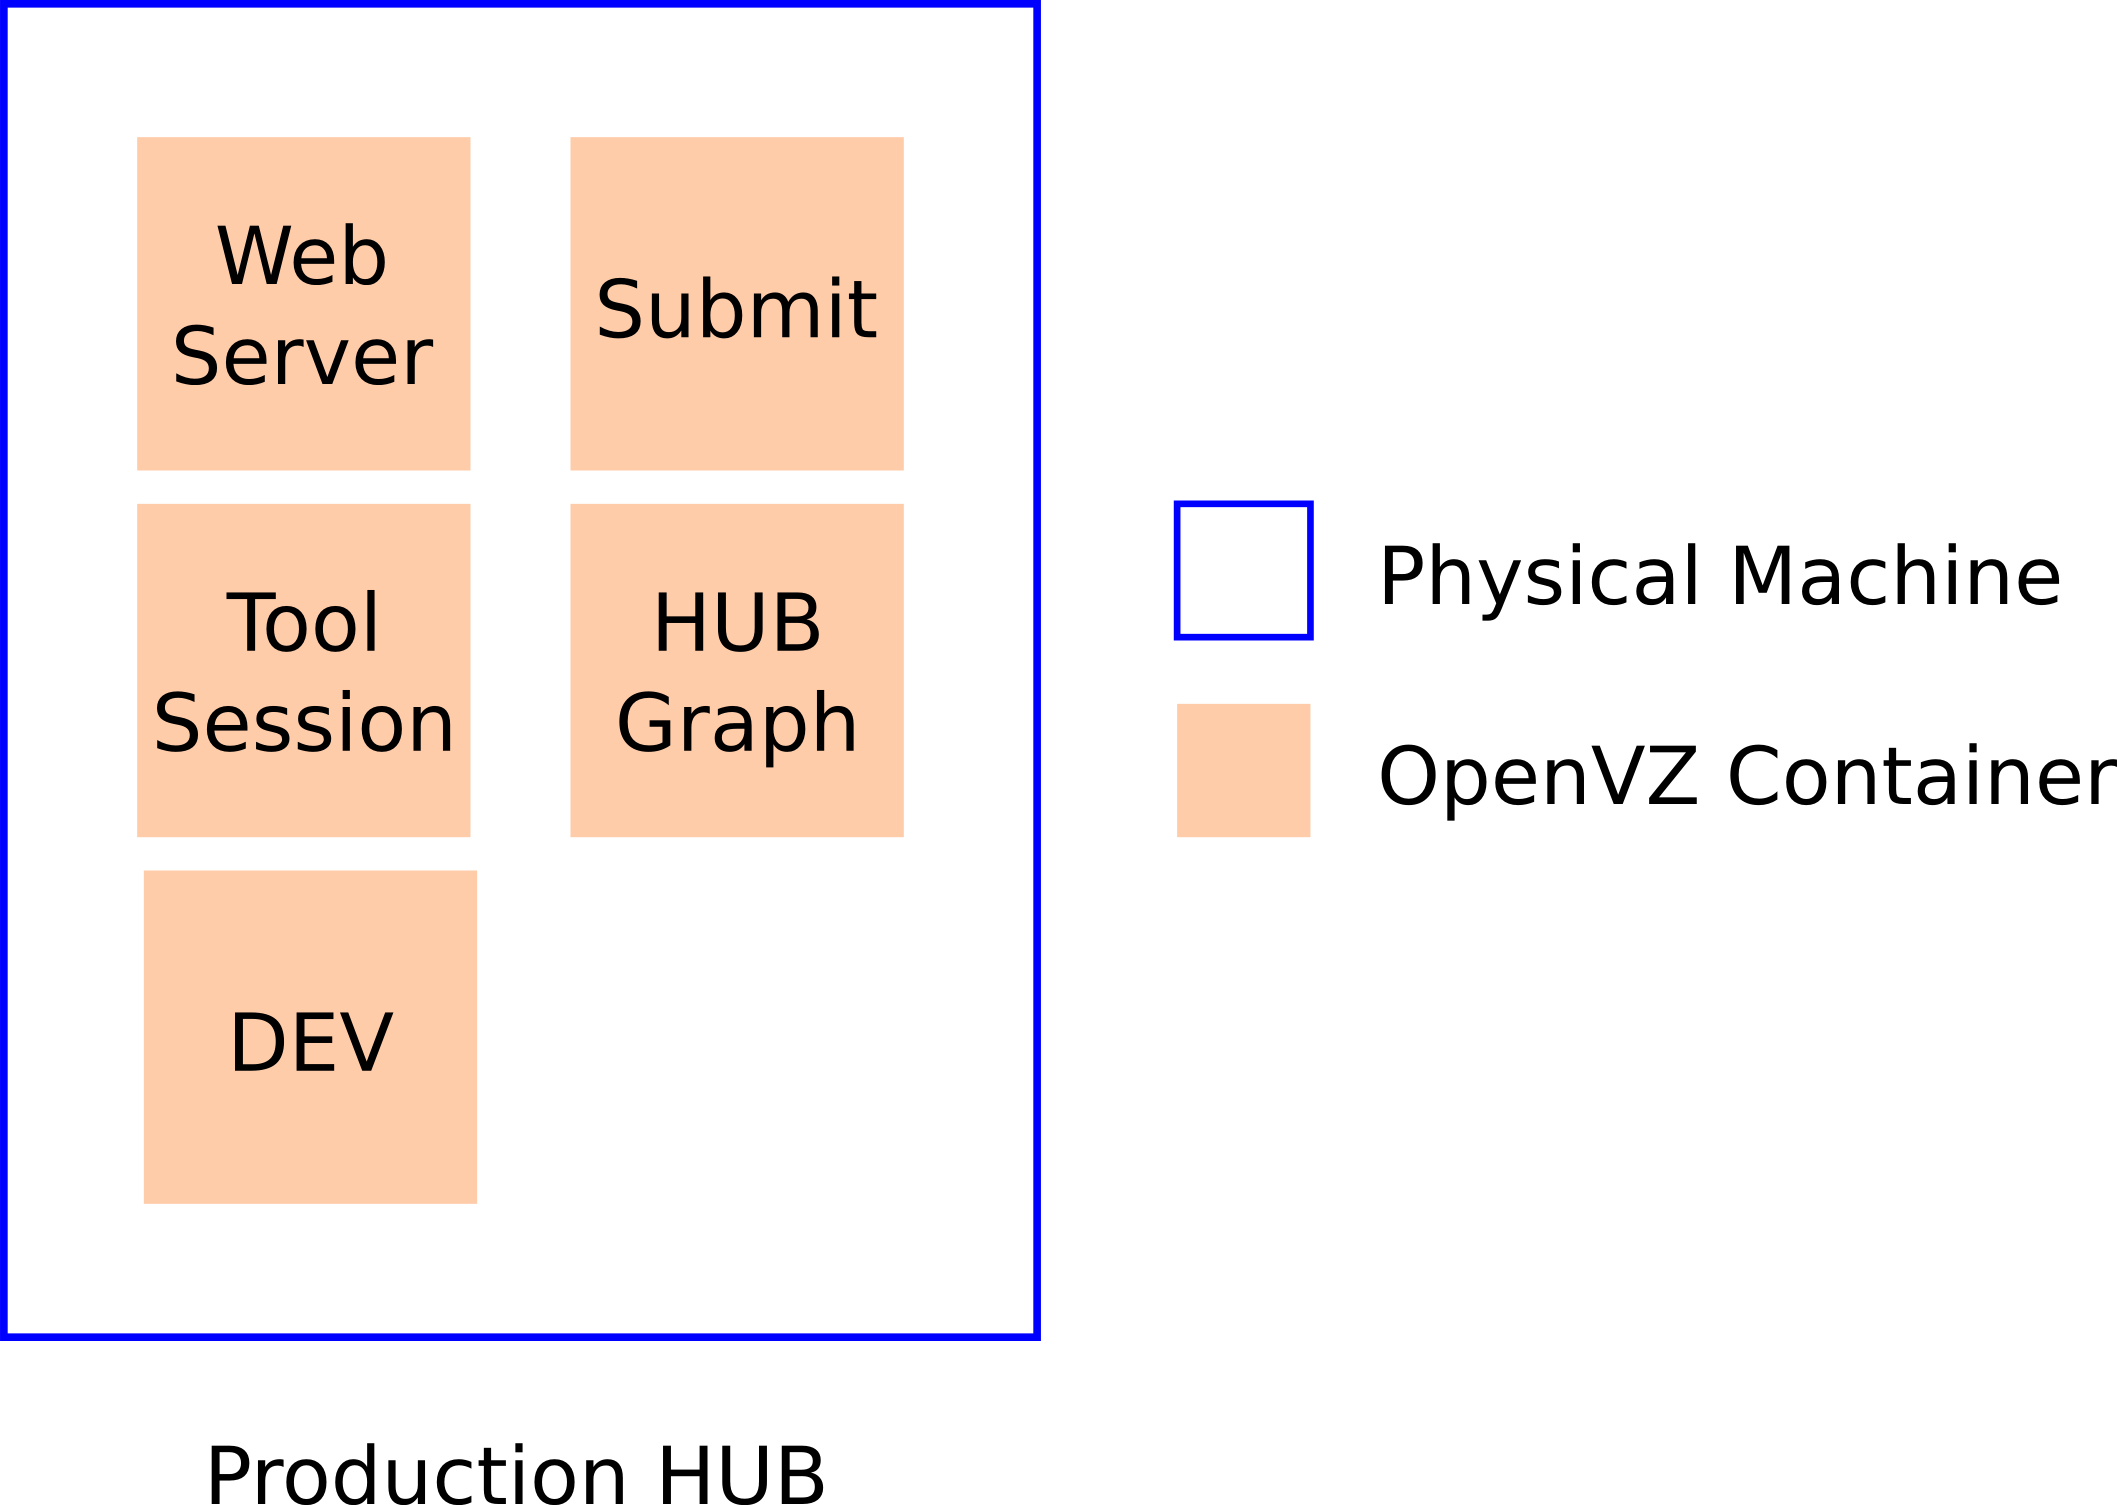
\includegraphics[width=0.5\textwidth]
    {../../images/qa_machine/proposed_setup_production.png}
  \caption{ Proposed layout of the testing environment using physical machines. }
\end{figure}

Hosting the test environment on physical machines in the same way a production
hub is hosted is the most basic way to build a test environment. This approach
has a number of drawbacks that make it an undesirable way to setup our
environment. Using a physical machine for each test environment is not a
scalable solution. It requires increasing amounts of rack space in the server
rooms and increases the number of managed physical machines.


\subsection{Virtual Machine}

\begin{figure}[ht!]
  \centering
  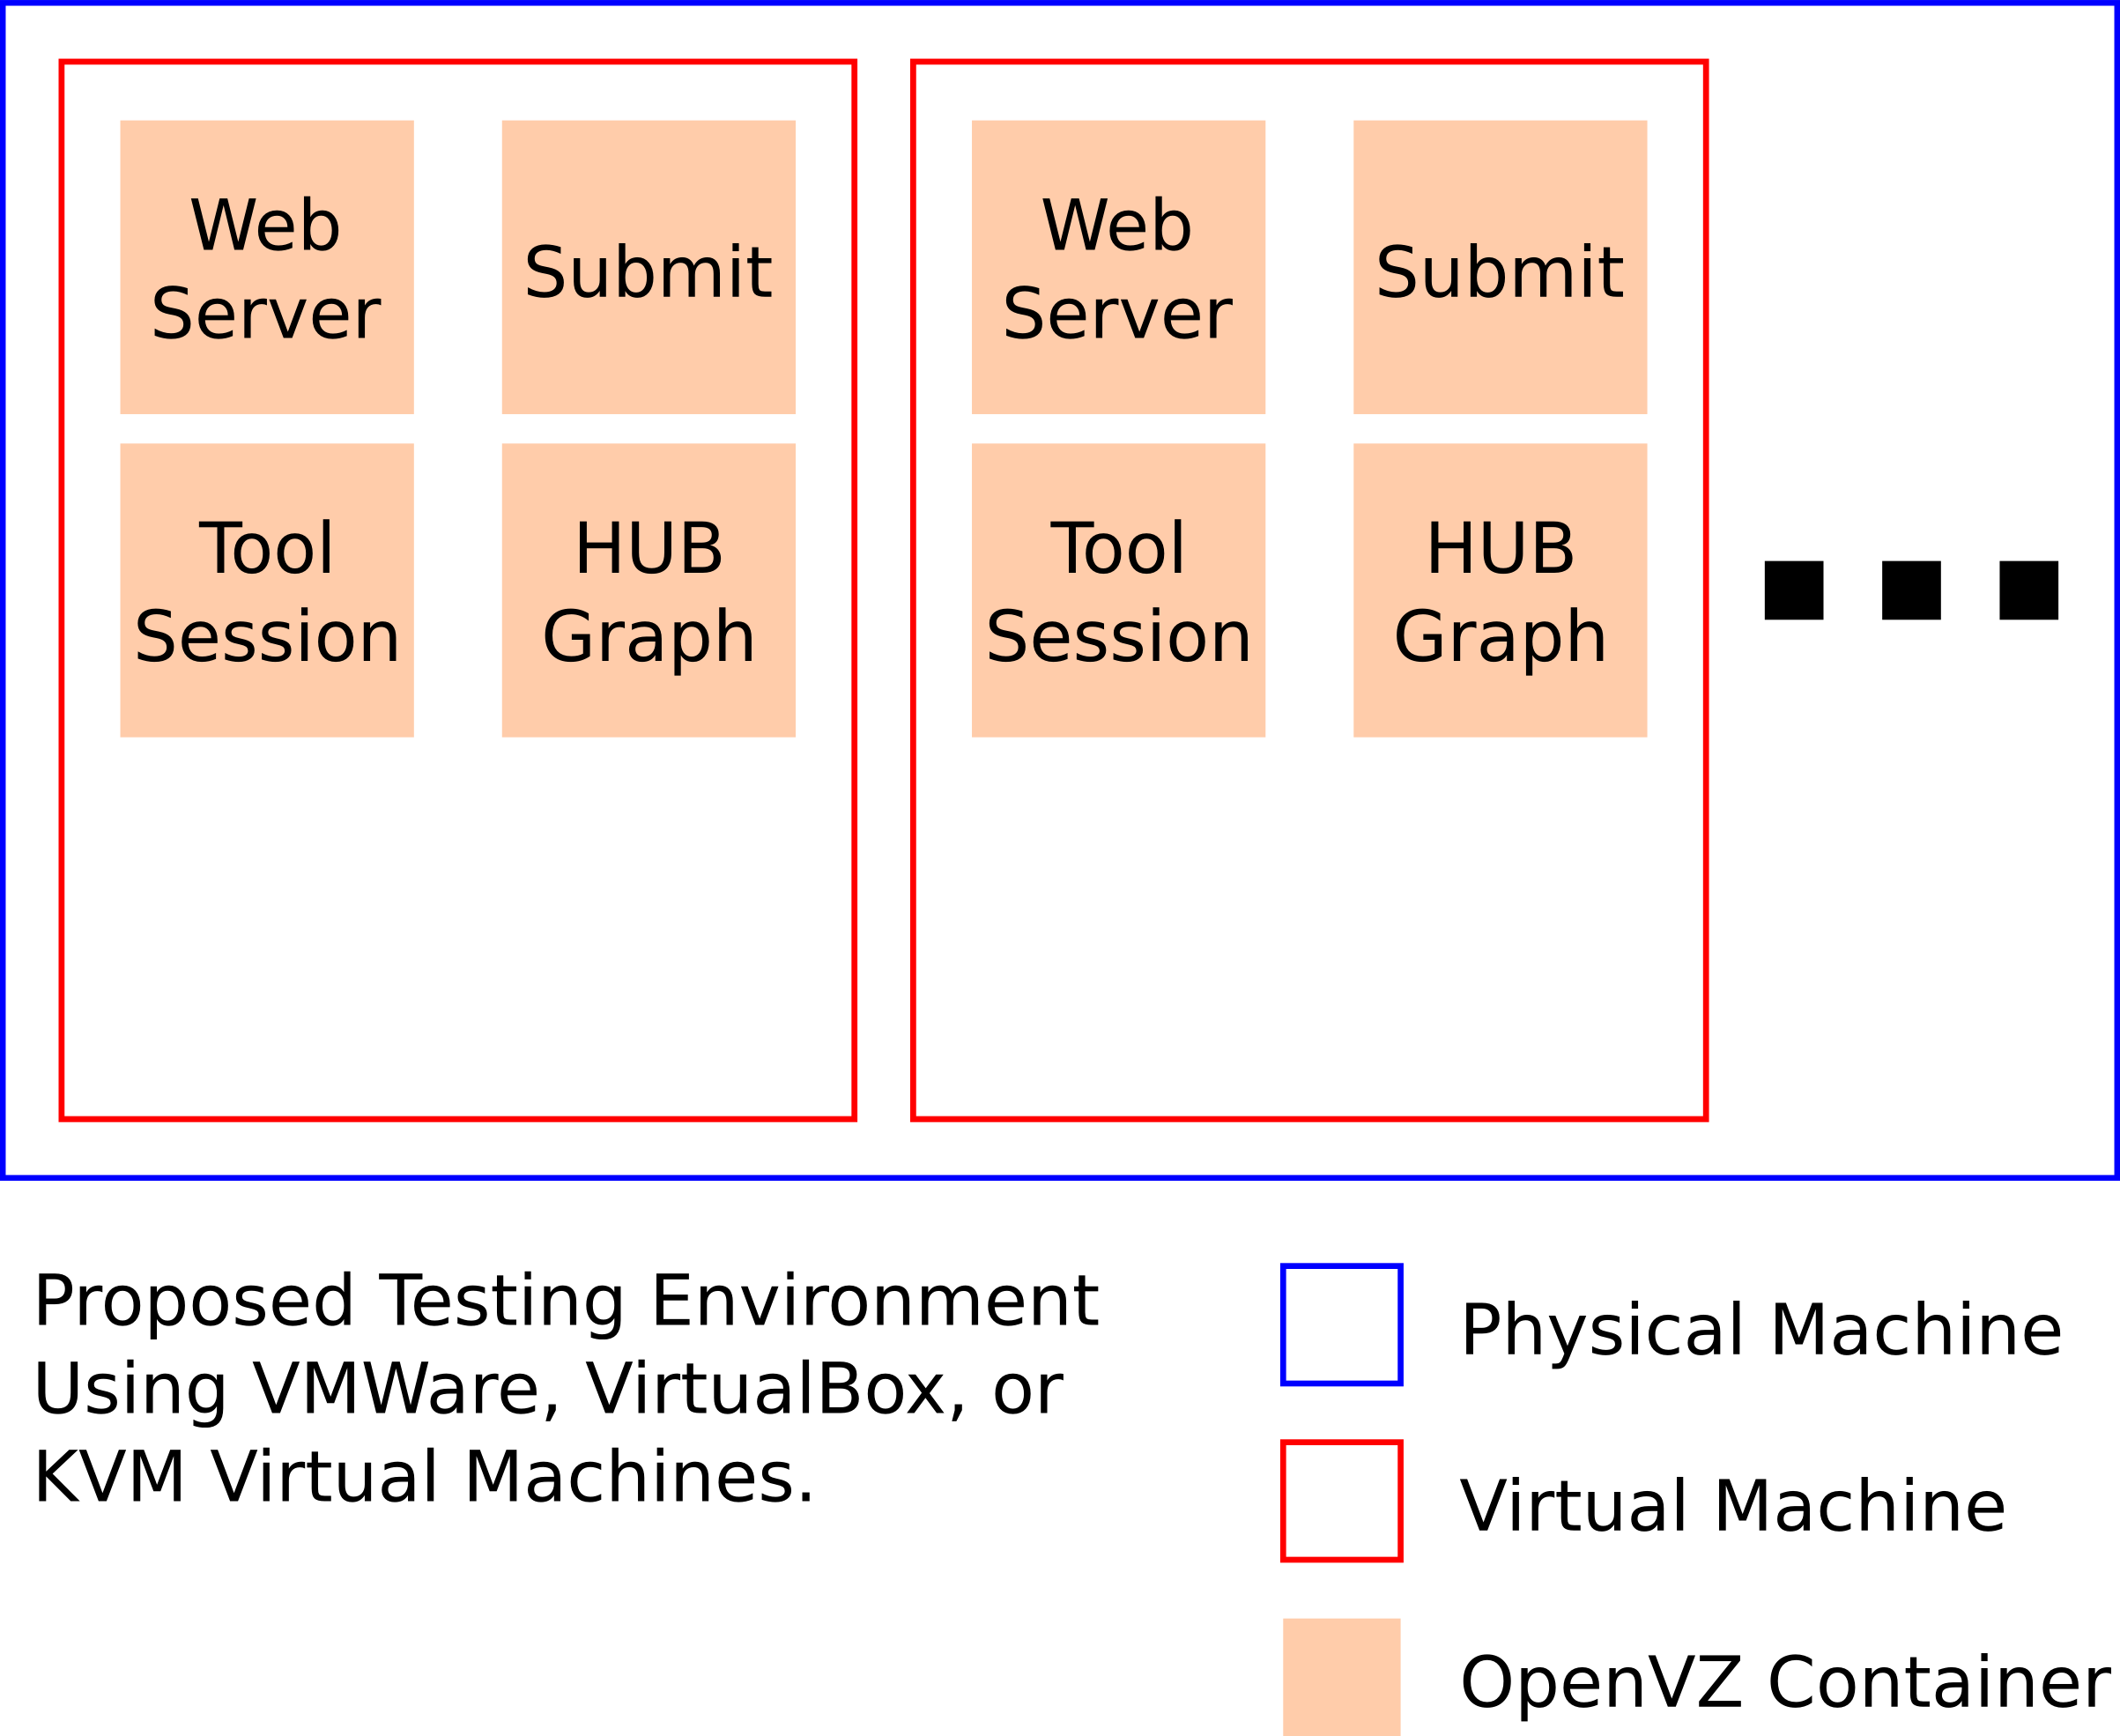
\includegraphics[width=0.5\textwidth]
    {../../images/qa_machine/proposed_setup_vm.png}
  \caption{ Proposed layout of the testing environment using virtual machines. }
\end{figure}

A more scalable setup is to use a virtual machine solution like VMWare,
VirtualBox, or Kernel-based Virtual Machine (KVM). This setup allows for
multiple test environments to exist on a single physical machine. Each test
environment can act as a proper \textit{hub-in-a-box}, supporting tool session
containers within the virtual environment. Virtual machines also support quick
cloning, refresh, and migration.

\subsection{OpenVZ}

\begin{figure}[ht!]
  \centering
  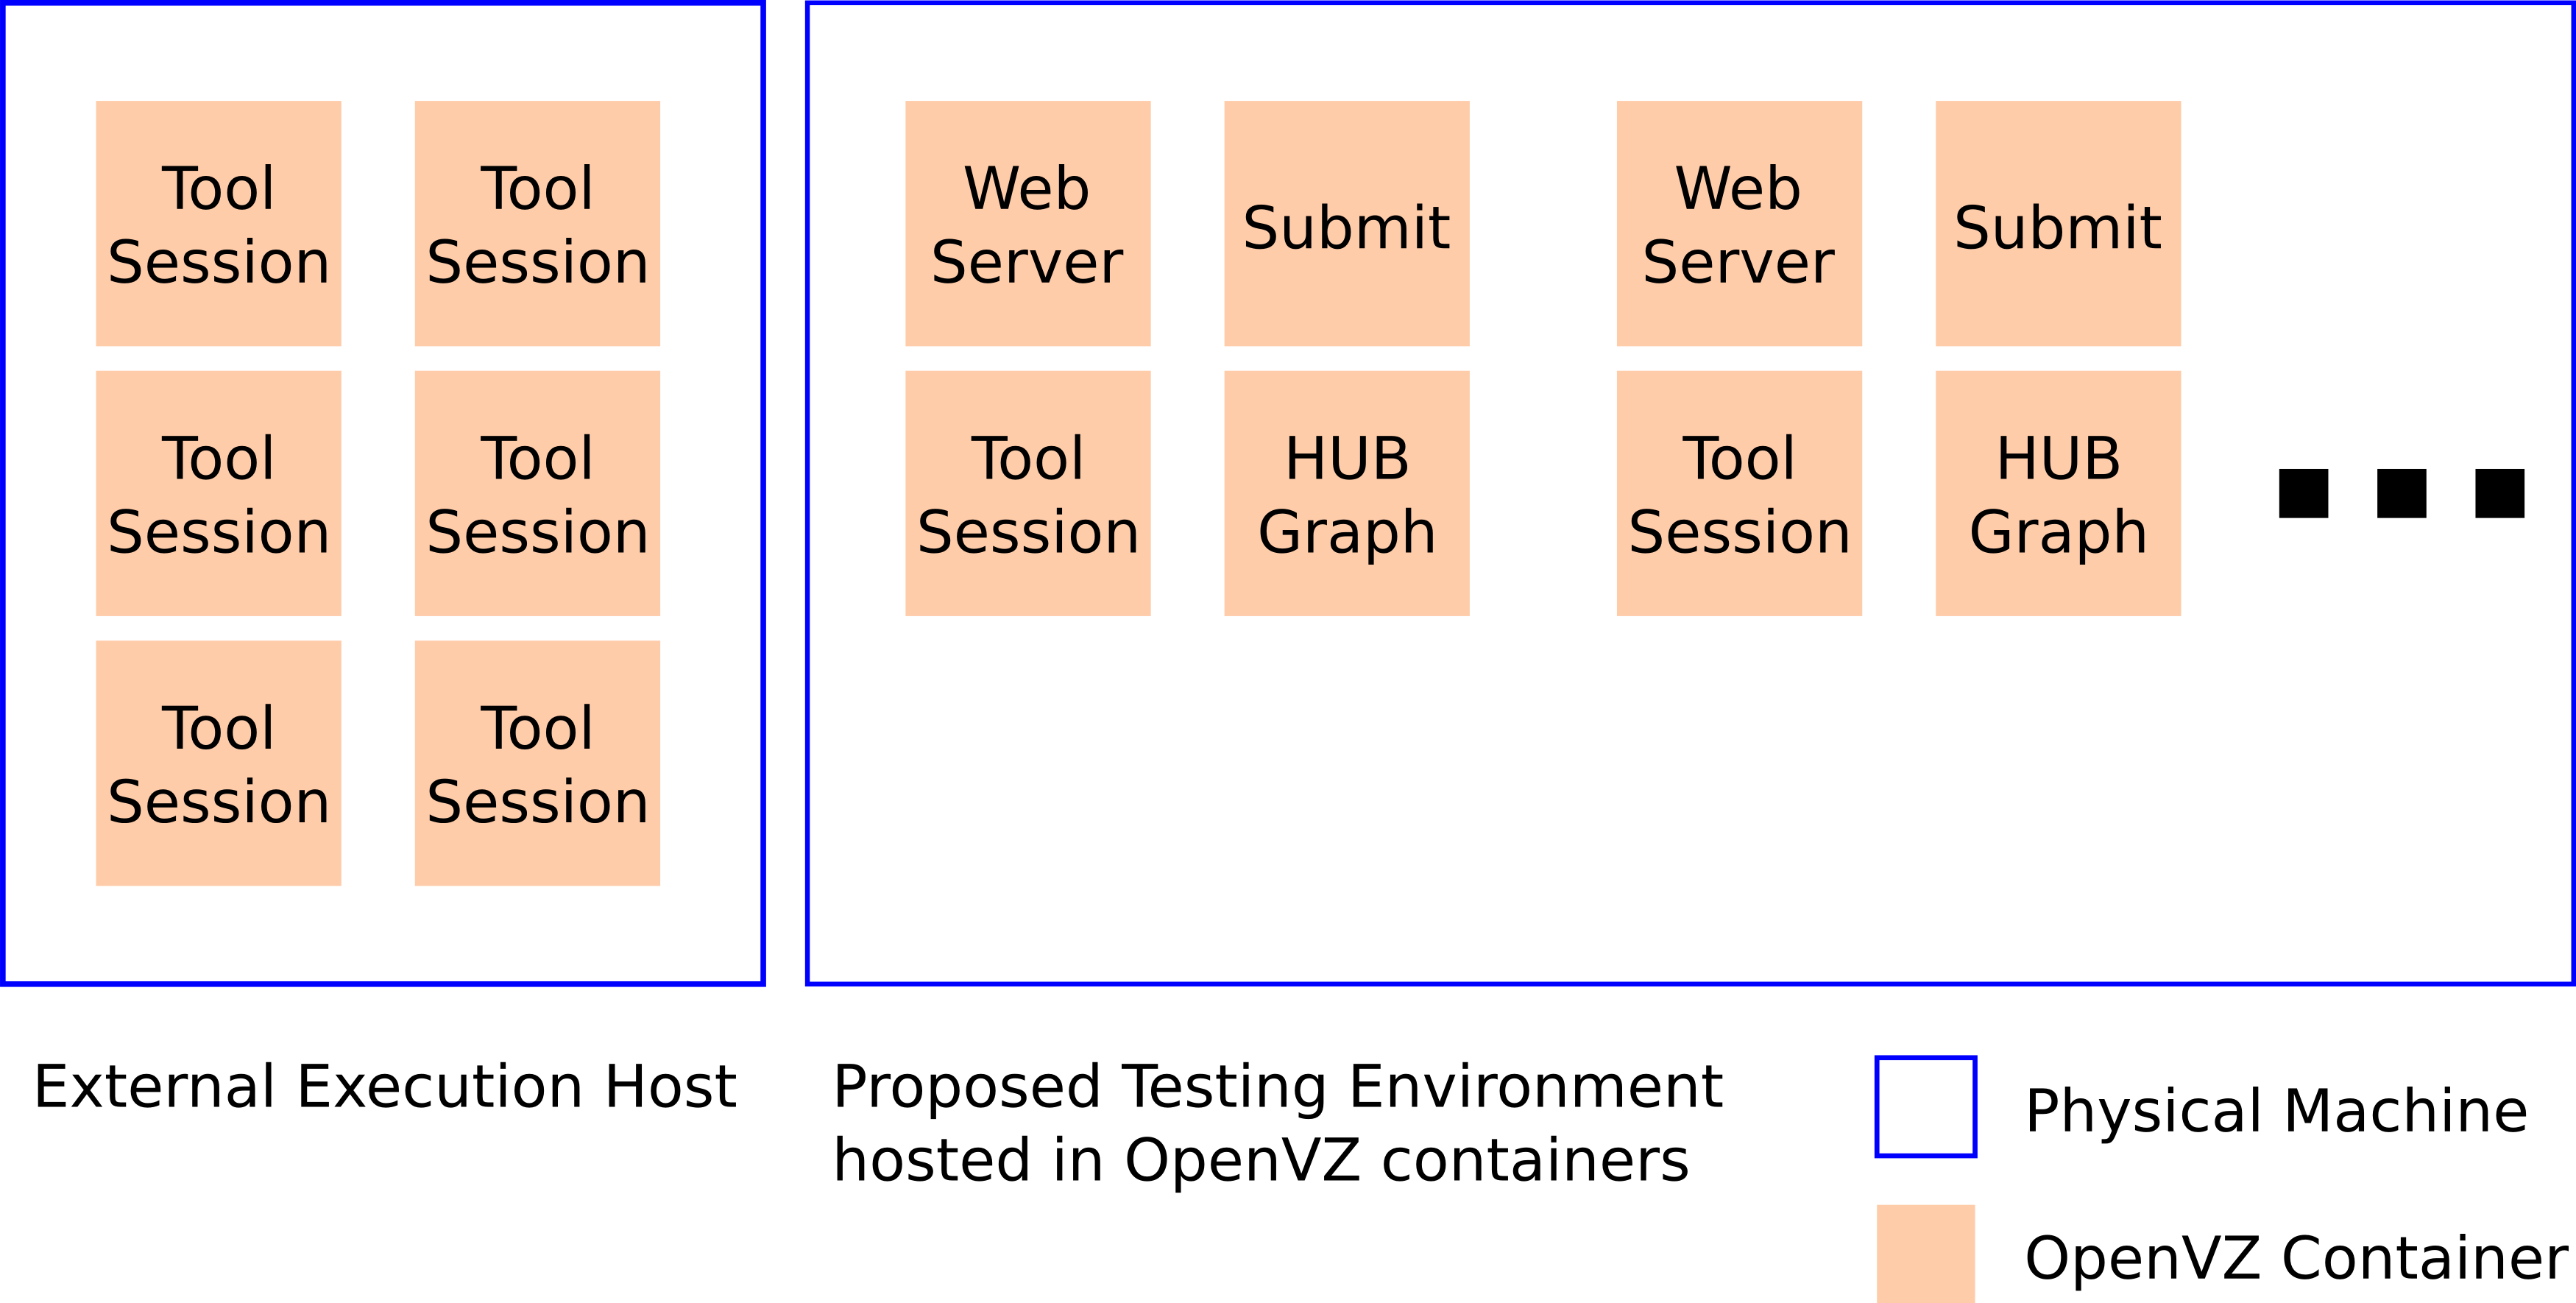
\includegraphics[width=0.75\textwidth]
    {../../images/qa_machine/proposed_setup_openvz.png}
  \caption{ Proposed layout of the testing environment using OpenVZ containers. }
\end{figure}

Another solution is to create test environments in OpenVZ containers on a
server.  Similar to the Virtual Machine solution, multiple test environment
could be hosted on a single server. The setup would need external execution
hosts associated with the test environments to be able to support launching
tool session containers. This solution resembles how some multi-machine hubs
are currently being hosted.


\section{Testing in the Environment}

Multiple testing environments will be available for use in parallel. When a new
piece of software needs to be tested before being included in the HUBzero
software stack, a new test environment will be instantiated with a clean
installation of the hub or pre-populated with data from a production hub. The
new software will be tested in the environment, with automated testing
scripts to check that the installation of the new software does not break other
components. The new software being tested should also have a set of test cases
that can be added to the automated test suite.

The general flow of testing a new piece of software in the environment will be
include the following steps:

\begin{enumerate}
\item Clean the machine of all hub software.
\item Load a known, previously tested version of the hub software.
\item Load the new piece of software to be tested.
\item Run general hub test cases to ensure the new software did not break other pieces of the hub.
\item Run software specific test cases to ensure the new software works properly within the hub environment.
\item If test cases failed, the developer can inspect and make changes to the testing environment. Repeat steps 1 - 5.
\item If test cases passed, create a new snapshot of the hub software, or integrate the new software into the HUBzero installation.
\end{enumerate}

The process for merging software from the testing environments back into the
HUBzero software stack is sequential.

\end{document}
